\chapter{Introduction}
With the rise of cloud-based clusters, developing robust distributed algorithms is becoming an increasingly difficult problem and the need for vigorous methodologies to verify the correctness of these algorithms has intensified. Modern programming languages have been developed to support distributed algorithms that rely on message-passing as a means of communication between sequential nodes executing in parallel. Common message-passing abstractions involve the use of channels (e.g. Go \cite{go}) or actors \cite{actor} (e.g. Erlang \cite{erlang}). Message-passing abstractions can be simple and more natural to reason about than a common alternative in shared-memory concurrency, however, it can also become more difficult to verify a program implements a given specification.
\par
Verification tools have been developed to support determining the correctness of systems. For example, first-order automated theorem provers such as Z3 \cite{z3} and formal specification languages like TLA+ \cite{tlaplus}. These tools allow systems to be modeled, and specifications to be defined that can then be used to prove properties over these systems. However, despite the power these tools provide, they often place a burden on developers to write and maintain models of systems alongside their actual implementation. This often leads to a paradigm shift away from system implementations that were designed in, for example, imperative programming languages such as C. Modern programming languages such as Dafny \cite{dafny} solve this issue by directly integrating Floyd-Hoare style logic verification alongside the implementation.
\par
Elixir \cite{elixir} is a functional programming language built on top of Erlang that runs on the BEAM virtual machine \cite{beam}. It is commonly used for building distributed, fault-tolerant applications because it supports concurrency, communication and distribution. Elixir actors are uniquely identified with a process identifier (pid) and associated with an unbounded mailbox. Each mailbox supports communication between actors; one actor can send a message to another actor's mailbox, which is then enqueued and can be received in a First-In-First-Firable-Out (FIFFO) ordering. FIFFO is similar to First-In-First-Out (FIFO) where elements are dequeued in the order they are enqueued, however, Elixir supports receiving messages with pattern-matching such that messages are received in a FIFO order concerning a certain pattern.
\par
This report discusses the modeling of actor-based programs and the verification of their adherence to a specification, using Elixir as a target language to support the verification of real-world systems.
\section{Objectives}
We introduce Verlixir, an analysis tool for Elixir programs and their adherence to formal properties specified in linear temporal logic. As a subsidiary, we introduce LTLixir, an extension to Elixir to support the specification and verification of actor-based systems. 
\par
Much work has gone into verifying algorithms and programs such as various theorem provers and model checkers. While these tools were initially designed to allow developers to write specifications for how an algorithm should behave in bespoke specification language, more recently verification tools have been designed that can be directly applied to programs written in programming languages such as C \cite{c_to_promela}. A more recent advancement is support for verifying concurrent programs, however much of this work has used global shared memory as an implementation for specifying process communication \cite{dafny_paper}. This project sets out to accomplish the following objectives:
\begin{itemize}
    \item Design novel abstraction techniques for modeling message-passing systems.
    \item Support in-line formal specifications alongside a modern programming language.
    \item Design a toolkit for simulation and verification of specifications of message-passing systems.
    \item Apply the aforementioned techniques and tooling to real-world systems implemented in Elixir.
\end{itemize}
The current research in the area of verifying modern programming languages presents many challenges for extending this notion to a message-passing system. State-of-the-art verification-aware languages such as Dafny avoid concurrent execution due to the challenges it can introduce to verification \cite{dafny_concurrency}. To verify a distributed system in this context, it is instead left to the user to model the system in a manner that it can be sequentially executed. Tools such as Gomela \cite{gomela} support verification of concurrent execution where communication is achieved across channels in Go, however, Go has a very different approach to the pure message-passing models we are interested in. We can draw a few comparisons between the two:
\begin{itemize}
    \item Go communication channels can be bounded, whereas Elixir mailboxes are unbounded. Naturally, unbounded queues can lead to more complex verification problems (state-space explosion).
    \item Go is statically typed, whereas Elixir is dynamically typed.
    \item Go has support for shared memory, Elixir's actor model strictly enforces all information sharing to be handled by message-passing.
\end{itemize}
These comparisons lead to challenge that need to be addressed in this report, however they are also reasons why Elixir is an interesting target language both for designing real-world systems and for verifying them.  
\section{Contributions}
To accomplish the objectives set out in this report, the following contributions have been made:
\begin{itemize}
    \item The primary contribution of this report is Verlixir. Verlixir is an analysis tool that parses Elixir programs and translates them into Promela \cite{promela} for model checking using the SPIN \cite{spin} model checker. Verlixir is capable of verifying multiple properties of highly concurrent Elixir programs and reporting back counterexamples in an Elixir-friendly format. Chapter \ref{chap:verlixir} provides an overview of what Verlixir is and how it can be used. We then provide a detailed explanation of the design and implementation of Verlixir in chapter \ref{chap:design}.
    \item The secondary contribution is LTLixir. LTLixir is a reduced subset of the standard Elixir language that has been extended to introduce linear temporal logic, predicate logic and a Floyd-Hoare style logic for specifying the behavior of a system alongside its implementation. Temporal properties specified in LTLixir can be verified using Verlixir. LTLixir is first introduced in section \ref{sec:ltlixir} and the design is discussed in section \ref{sec:specification_language}.
\end{itemize}
Figure \ref{fig:overview_dig} shows where these components fit into the existing Elixir toolchain.
\begin{figure}[H]
    \centering
    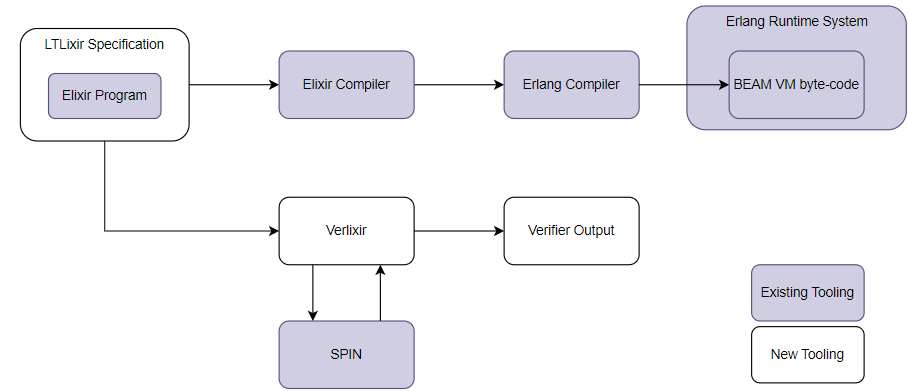
\includegraphics[width=0.8\textwidth]{images/high_level_system.png}
    \caption{High-level diagram of the verification-aware Elixir toolchain.}
    \label{fig:overview_dig}
\end{figure}